\chapter{Methodology and System Design}
\label{chap:system-design}

\section{High-Level Architectural Topology}
\label{sec:arch-overview}

The MergeMind architecture is structured as a resilient, enterprise-grade modular monolith that balances rapid developer feedback, deterministic execution isolation, and scalable external service integrations. The platform comprises four primary operational tiers:

\begin{enumerate}
    \item \textbf{Presentation Tier (Client SPA):} Implemented using React 18, TypeScript, Vite, and Tailwind CSS, providing a responsive, low-latency single-page application for repository health exploration, security posture compliance, pull request analysis, and remediation diff inspection.
    \item \textbf{Application and Routing Tier (FastAPI Backend):} Built on Python 3.11 and the asynchronous FastAPI web framework, serving as the centralized business logic orchestration layer, API gateway, cryptographic authenticator, and webhook handler.
    \item \textbf{Relational Persistence Tier (PostgreSQL 18):} An enterprise ACID-compliant relational database accessed via SQLAlchemy 2.0 ORM and Asyncpg, managing repository metadata, health snapshots, CI failure traces, AI remediation proposals, and audit logs.
    \item \textbf{Sandboxed Execution and AI Intelligence Tier:} Comprising isolated ephemeral Docker execution containers for code evaluation and regression verification, combined with the Google Gemini 3.6 Flash generative API for automated code reasoning, stack trace triage, and unified diff synthesis.
\end{enumerate}

Figure~\ref{fig:overall-architecture} illustrates the overarching multi-tier system topology and data flow pathways across all system layers.

\begin{figure}[htbp]
    \centering
    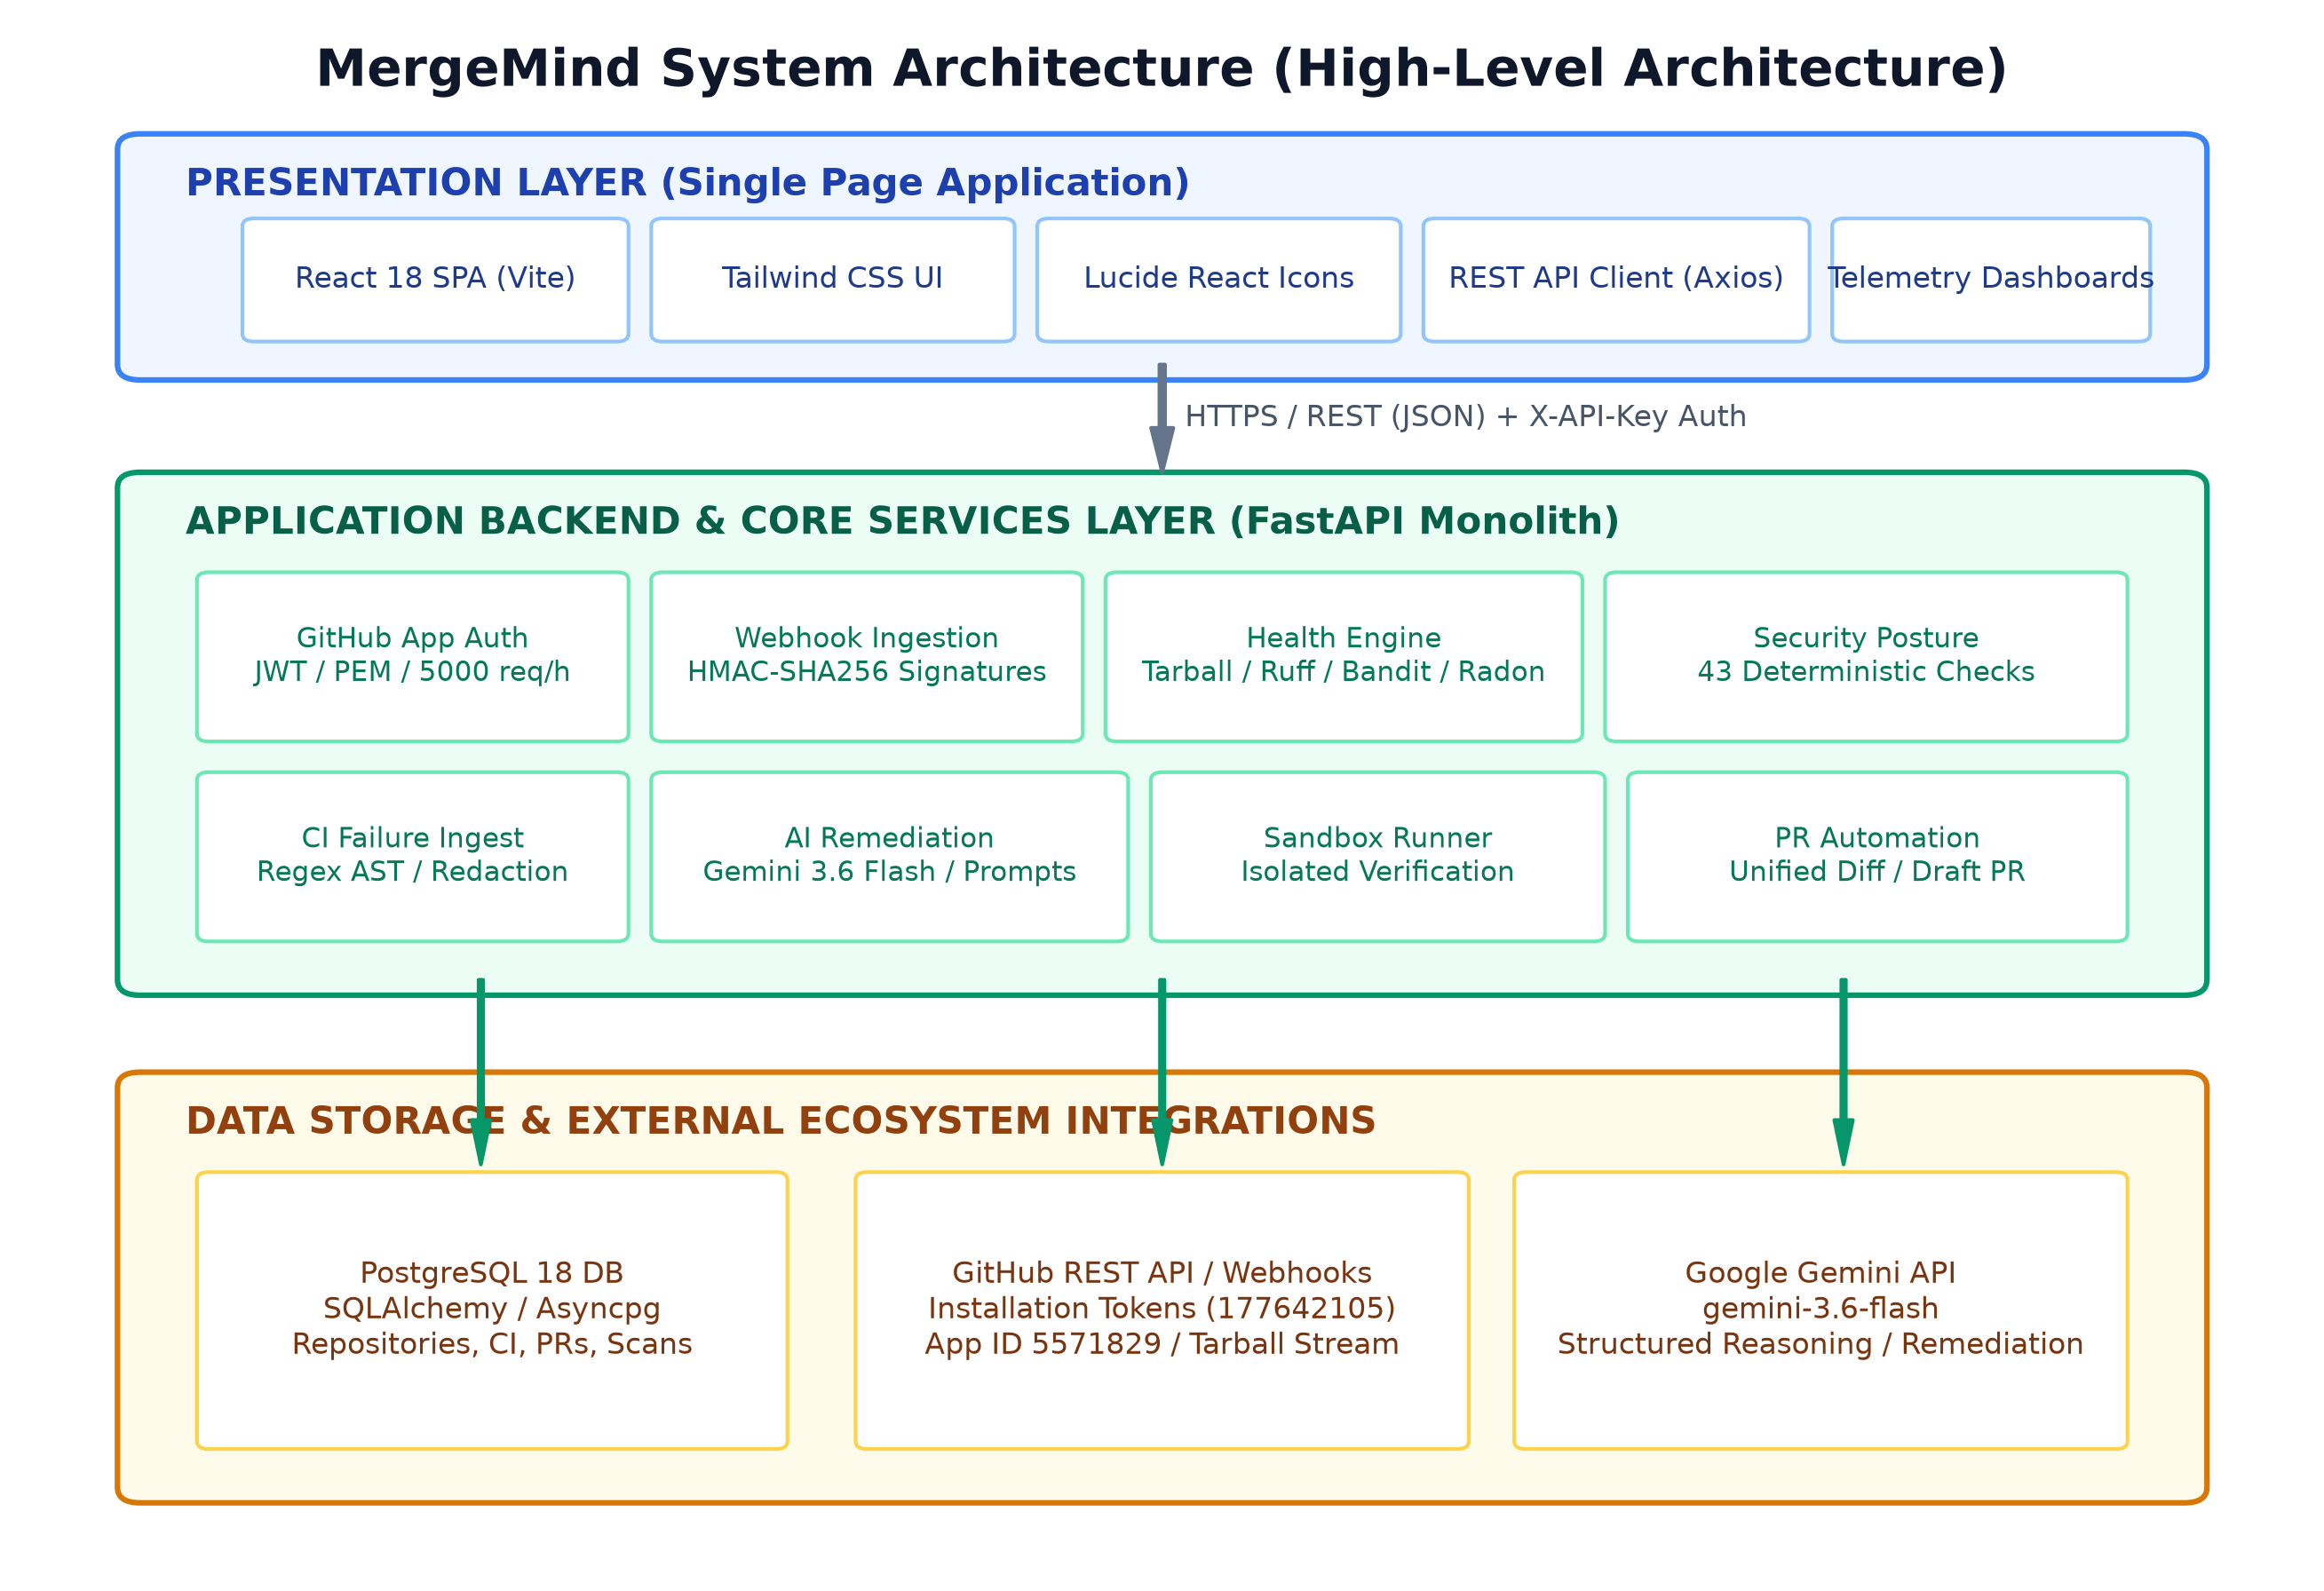
\includegraphics[width=0.92\textwidth]{images/architecture/overall_architecture.png}
    \caption{MergeMind High-Level System Architecture and Multi-Tier Topology}
    \label{fig:overall-architecture}
\end{figure}

\section{System Actor Profiles and Operational Use Cases}
\label{sec:use-cases}

MergeMind interacts with three primary actors: Software Developers, DevSecOps Engineers, and External Systems (GitHub App and GitHub Actions CI Runners). Figure~\ref{fig:use-case-diagram} models the system's operational use-case boundaries.

\begin{figure}[htbp]
    \centering
    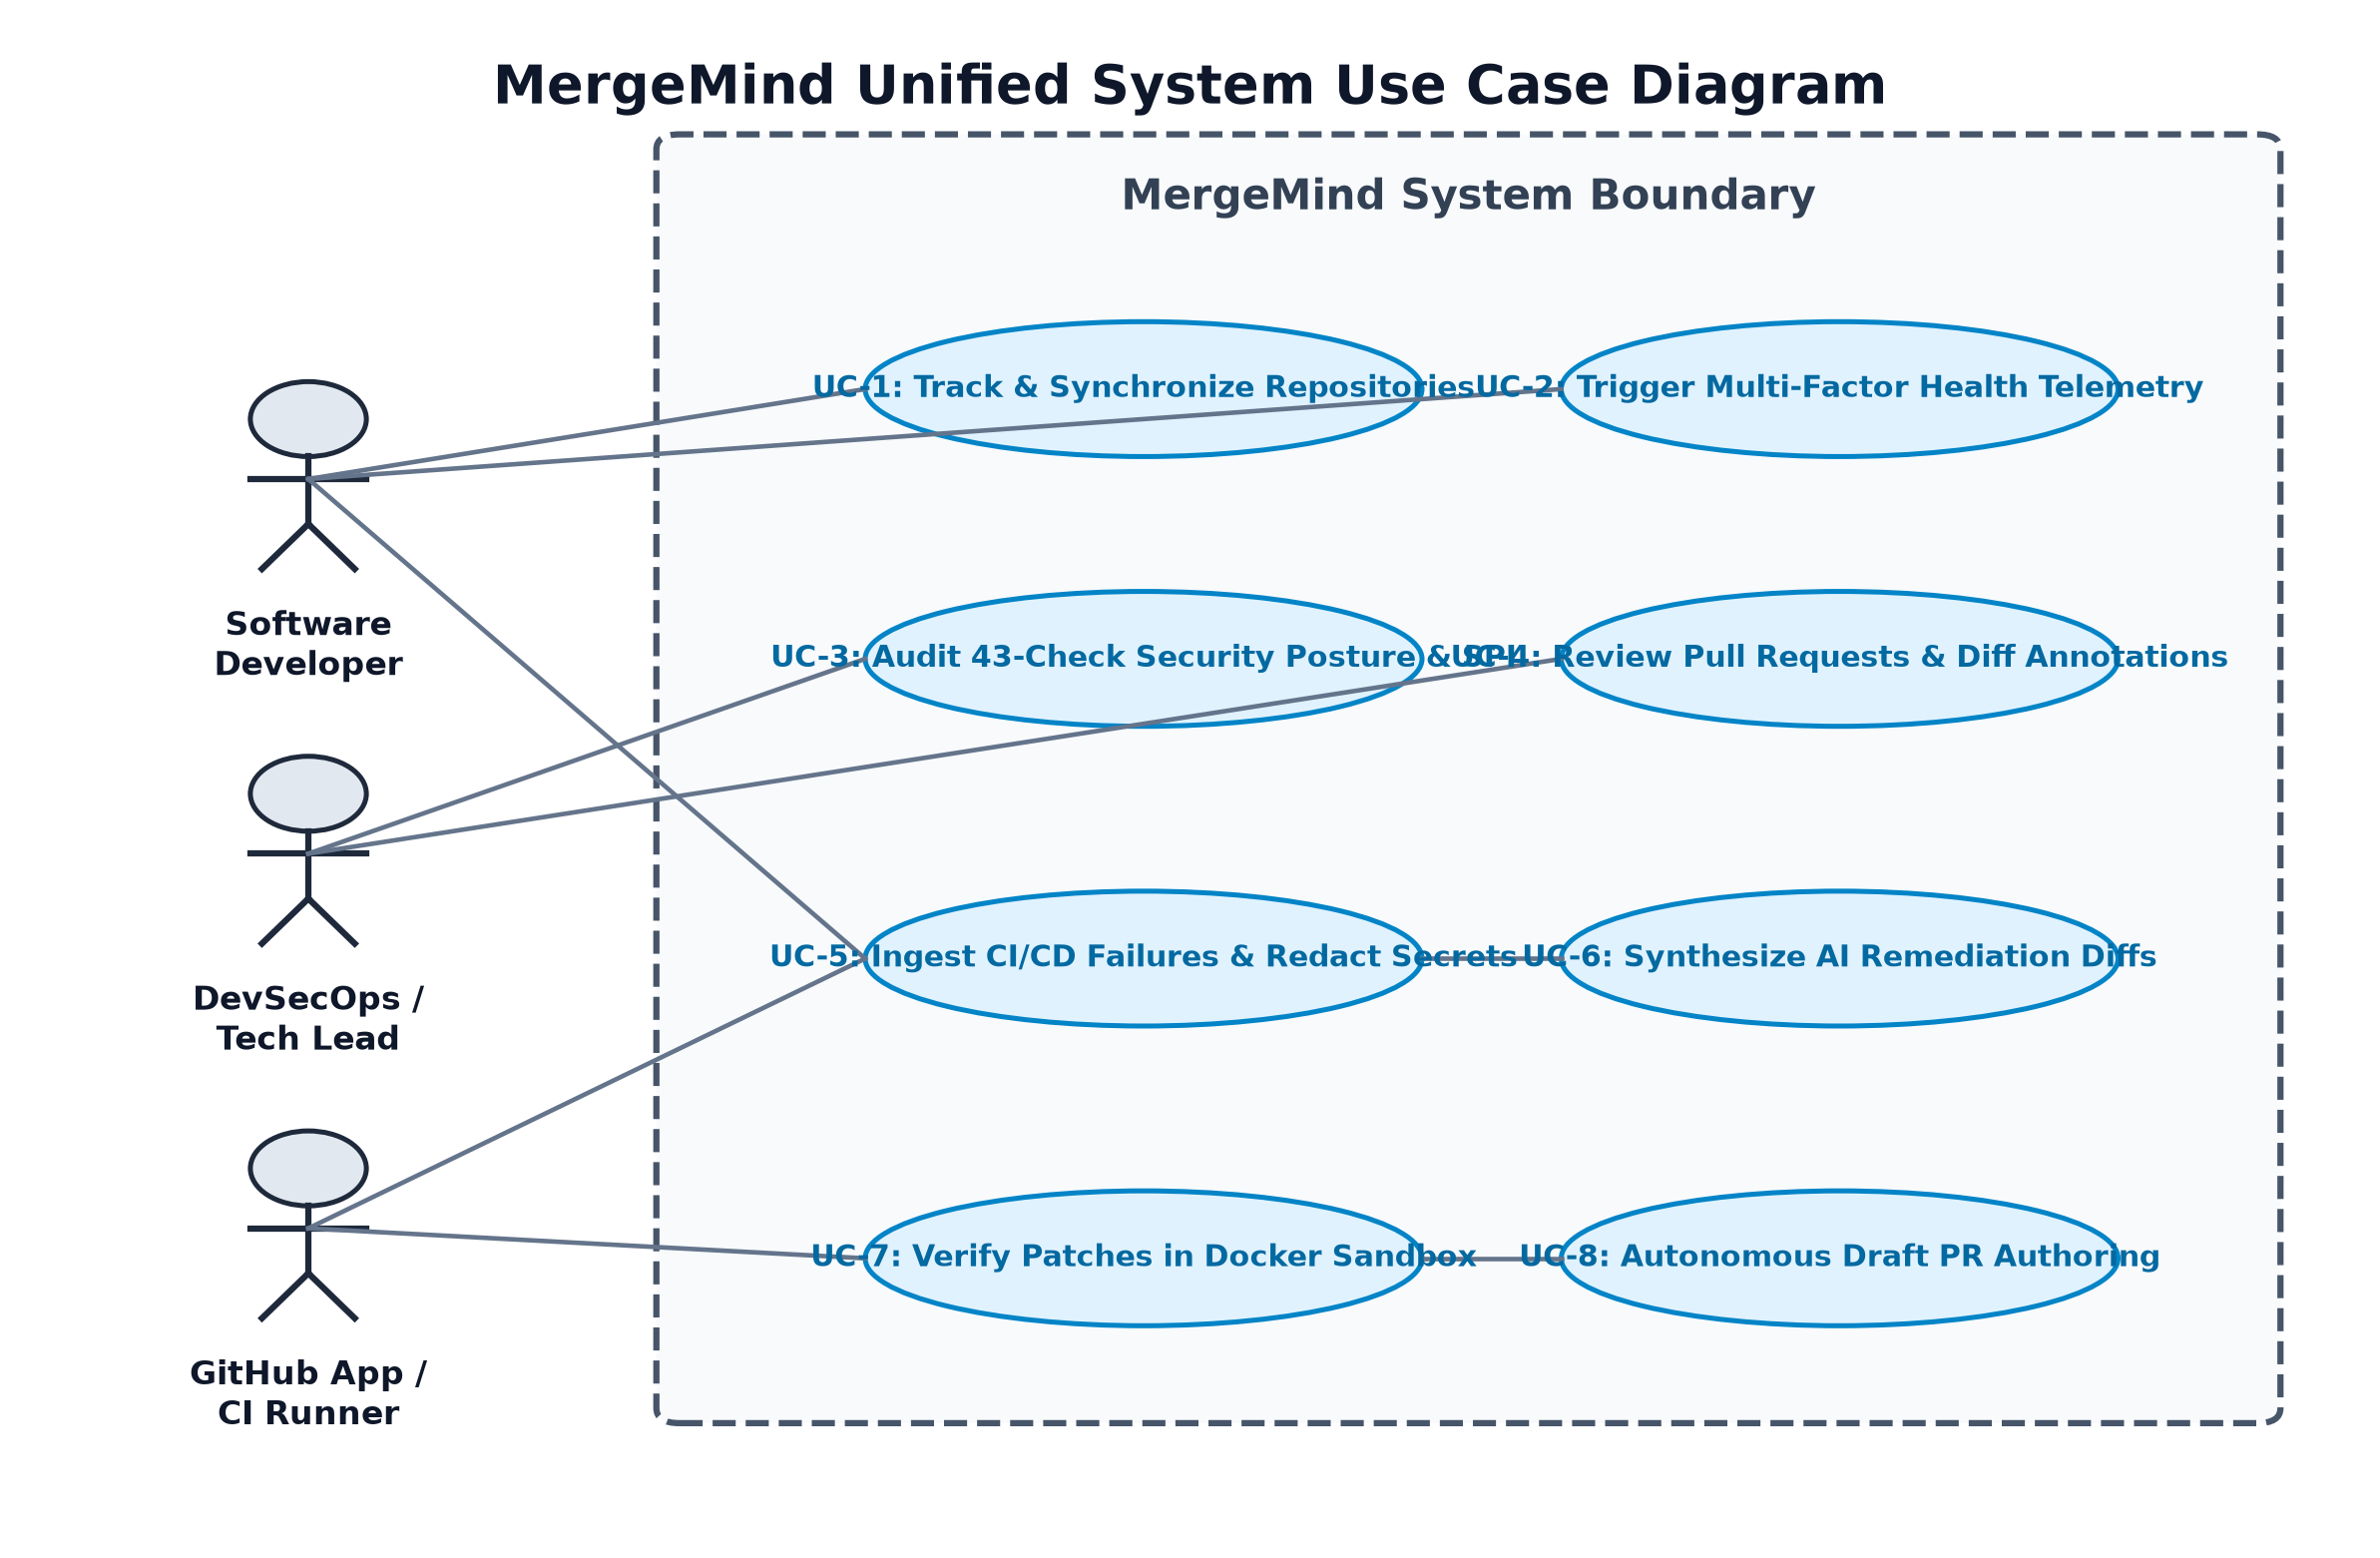
\includegraphics[width=0.88\textwidth]{images/diagrams/use_case_diagram.png}
    \caption{MergeMind Unified System Use Case Diagram}
    \label{fig:use-case-diagram}
\end{figure}

\section{Functional Requirements Specification}
\label{sec:functional-reqs}

Table~\ref{tab:functional-requirements} specifies the formal functional requirements implemented across all platform subsystems.

\begin{longtable}{p{0.14\textwidth} p{0.26\textwidth} p{0.54\textwidth}}
\caption{Comprehensive Functional Requirements Specification (FR-01 to FR-16)} \label{tab:functional-requirements} \\
\toprule
\textbf{Req. ID} & \textbf{Subsystem Module} & \textbf{Operational Requirement Specification} \\
\midrule
\endfirsthead
\toprule
\textbf{Req. ID} & \textbf{Subsystem Module} & \textbf{Operational Requirement Specification} \\
\midrule
\endhead
\bottomrule
\endfoot
\bottomrule
\endlastfoot

FR-01 & GitHub Authenticator & Mint short-lived RS256 JWTs using private RSA PEM keys to obtain installation access tokens with 5,000 req/hr rate limits. \\
\addlinespace
FR-02 & Webhook Receiver & Ingest GitHub HTTP webhooks, verify HMAC-SHA256 signatures, and asynchronously dispatch push, pull\_request, and workflow\_run events. \\
\addlinespace
FR-03 & Tarball Ingestion & Stream target repository tarball archives from GitHub REST API and decompress into ephemeral sandboxed temporary directories. \\
\addlinespace
FR-04 & Code Quality Scanner & Execute Astral Ruff across ingested source files, computing an objective 0--100 Code Quality score (Weight: 25\%). \\
\addlinespace
FR-05 & Static Security Scanner & Execute Bandit AST security analysis, classifying findings by Severity/Confidence and computing an objective 0--100 Security score (Weight: 25\%). \\
\addlinespace
FR-06 & Dependency Scanner & Execute pip-audit against project dependency manifests, mapping pinned packages against known CVEs (Weight: 20\%). \\
\addlinespace
FR-07 & Complexity Scanner & Execute Radon AST traversal, calculating McCabe cyclomatic complexity and Maintainability Index scores (Weight: 10\%). \\
\addlinespace
FR-08 & Test Health Scanner & Execute Pytest test runners inside isolated environments, recording test pass rate and code coverage metrics (Weight: 20\%). \\
\addlinespace
FR-09 & Dynamic Calibration & Re-normalize total health score dynamically when optional tools are unconfigured, ensuring unbiased health evaluations. \\
\addlinespace
FR-10 & Qualification Gating & Gate repository health classification: assign QUALIFIED status only when assessment completeness reaches $\ge 80\%$ with primary linters active. \\
\addlinespace
FR-11 & Security Posture Audit & Execute 43 deterministic policy checks across Branch Protection (12), Security Features (9), Access Control (8), and Repo Settings (14). \\
\addlinespace
FR-12 & CI Failure Ingestion & Ingest raw CI build/test failure logs, reconciling raw\_log/raw\_logs payloads and redacting sensitive credentials via regex filters. \\
\addlinespace
FR-13 & Stack Frame Localizer & Parse assertion error traces and stack frames using regex AST matching to identify target source file, line number, and broken symbol. \\
\addlinespace
FR-14 & AI Diff Synthesis & Construct structured prompts to Google Gemini 3.6 Flash, enforcing unified diff output format adhering to standard patch specifications. \\
\addlinespace
FR-15 & Sandbox Verification & Apply AI unified diff inside an isolated ephemeral Docker container sandbox and re-execute Pytest test suites to verify fix validity. \\
\addlinespace
FR-16 & Draft PR Authoring & Upon sandbox verification pass, authenticate via GitHub App to create an automated Draft Pull Request containing patch diff and AI reasoning. \\
\end{longtable}

\section{Non-Functional Requirements Specification}
\label{sec:non-functional-reqs}

Table~\ref{tab:non-functional-requirements} details the architectural quality attributes, performance constraints, and security guarantees enforced by MergeMind.

\begin{table}[htbp]
    \centering
    \caption{Non-Functional Requirements Specification (NFR-01 to NFR-08)}
    \label{tab:non-functional-requirements}
    \small
    \begin{tabularx}{\textwidth}{p{0.14\textwidth} p{0.24\textwidth} p{0.56\textwidth}}
        \toprule
        \textbf{Req. ID} & \textbf{Quality Dimension} & \textbf{Guaranteed Quality Standard \& Target Metric} \\
        \midrule
        NFR-01 & Security \& Privacy & All raw CI logs and LLM prompts must undergo regex secret scrubbing before transmission. Asymmetric RSA keys must reside with 400 file permissions. \\
        \addlinespace
        NFR-02 & Determinism & Given the identical commit SHA and environment state, static health scoring algorithms must produce 100\% reproducible numerical outputs. \\
        \addlinespace
        NFR-03 & Sandbox Isolation & Remediation patch testing must execute within unprivileged Docker containers with dropped capabilities, bounded CPU/RAM, and no host volume mounts. \\
        \addlinespace
        NFR-04 & Latency & Read endpoints (GET health-assessment, GET security-posture) must respond in $< 150$ms under cached conditions and $< 4.0$s during live tarball extraction. \\
        \addlinespace
        NFR-05 & Quota Resilience & GitHub REST API requests must automatically utilize GitHub App installation tokens, maintaining a 5,000 req/hr quota with automated backoff retry. \\
        \addlinespace
        NFR-06 & Schema Robustness & CI failure ingestion endpoints must accept diverse CI payload schemas (raw\_log, raw\_logs) without raising 422 Unprocessable Entity errors. \\
        \addlinespace
        NFR-07 & Concurrency & Relational database must enforce foreign key integrity and transactional isolation across asynchronous concurrent webhook ingestions. \\
        \addlinespace
        NFR-08 & Ergonomics & Frontend SPA must provide responsive layout across desktop and tablet viewports, rendering telemetry dashboards and code diffs without UI lag. \\
        \bottomrule
    \end{tabularx}
\end{table}

\section{Multi-Factor Health Telemetry Scoring Methodology}
\label{sec:health-methodology}

Rather than relying on qualitative letter grades, MergeMind models repository health as a bounded mathematical function evaluating five orthogonal software engineering dimensions:

Let $D = \{d_1, d_2, d_3, d_4, d_5\}$ represent the five evaluation dimensions:
\begin{itemize}
    \item $d_1$: Code Quality and Stylistic Conformance (Astral Ruff), with nominal weight $W_1 = 25\%$
    \item $d_2$: Static AST Security Vulnerability Posture (Bandit), with nominal weight $W_2 = 25\%$
    \item $d_3$: Dependency Software Supply Chain Hygiene (pip-audit), with nominal weight $W_3 = 20\%$
    \item $d_4$: Cyclomatic Complexity and Maintainability (Radon), with nominal weight $W_4 = 10\%$
    \item $d_5$: Test Suite Health and Pass Rate (Pytest), with nominal weight $W_5 = 20\%$
\end{itemize}

Each dimension produces a bounded sub-score $S_i \in [0, 100]$. The nominal composite score $S_{\text{nominal}}$ is:

\begin{equation}
S_{\text{nominal}} = \sum_{i=1}^{5} (W_i \cdot S_i), \quad \text{where } \sum_{i=1}^{5} W_i = 100\%
\label{eq:nominal-health-score}
\end{equation}

\subsection{Dynamic Re-Normalization Engine for Partial Tooling}
In real-world repositories, certain tools may be unconfigured (e.g., missing dependencies manifest or absent test suites). Setting unconfigured dimensions to 0 would unfairly penalize clean repositories. MergeMind solves this through dynamic weight re-normalization. Let $A \subseteq \{1, 2, 3, 4, 5\}$ represent the set of active dimensions. Assessment Completeness $C$ is:

\begin{equation}
C = \frac{\sum_{i \in A} W_i}{100.0}
\label{eq:completeness}
\end{equation}

The final composite Health Score $S_{\text{final}}$ is dynamically re-normalized exclusively over active weights:

\begin{equation}
S_{\text{final}} = \frac{\sum_{i \in A} (W_i \cdot S_i)}{\sum_{i \in A} W_i}
\label{eq:renormalized-health-score}
\end{equation}

\subsection{Authoritative Qualification Gating}
A score derived from only one linter lacks statistical completeness. MergeMind enforces Authoritative Qualification Gating:
\begin{itemize}
    \item \textbf{QUALIFIED:} Assigned if and only if $C \ge 0.80$ (at least 80\% of nominal weights evaluated) and core baseline linters (Ruff and Bandit) execute successfully without runtime errors.
    \item \textbf{PROVISIONAL:} If $C < 0.80$, the score is classified as PROVISIONAL, alerting developers that additional tool configurations are necessary for authoritative evaluation.
\end{itemize}

Figure~\ref{fig:health-workflow} illustrates the end-to-end multi-factor health telemetry workflow.

\begin{figure}[htbp]
    \centering
    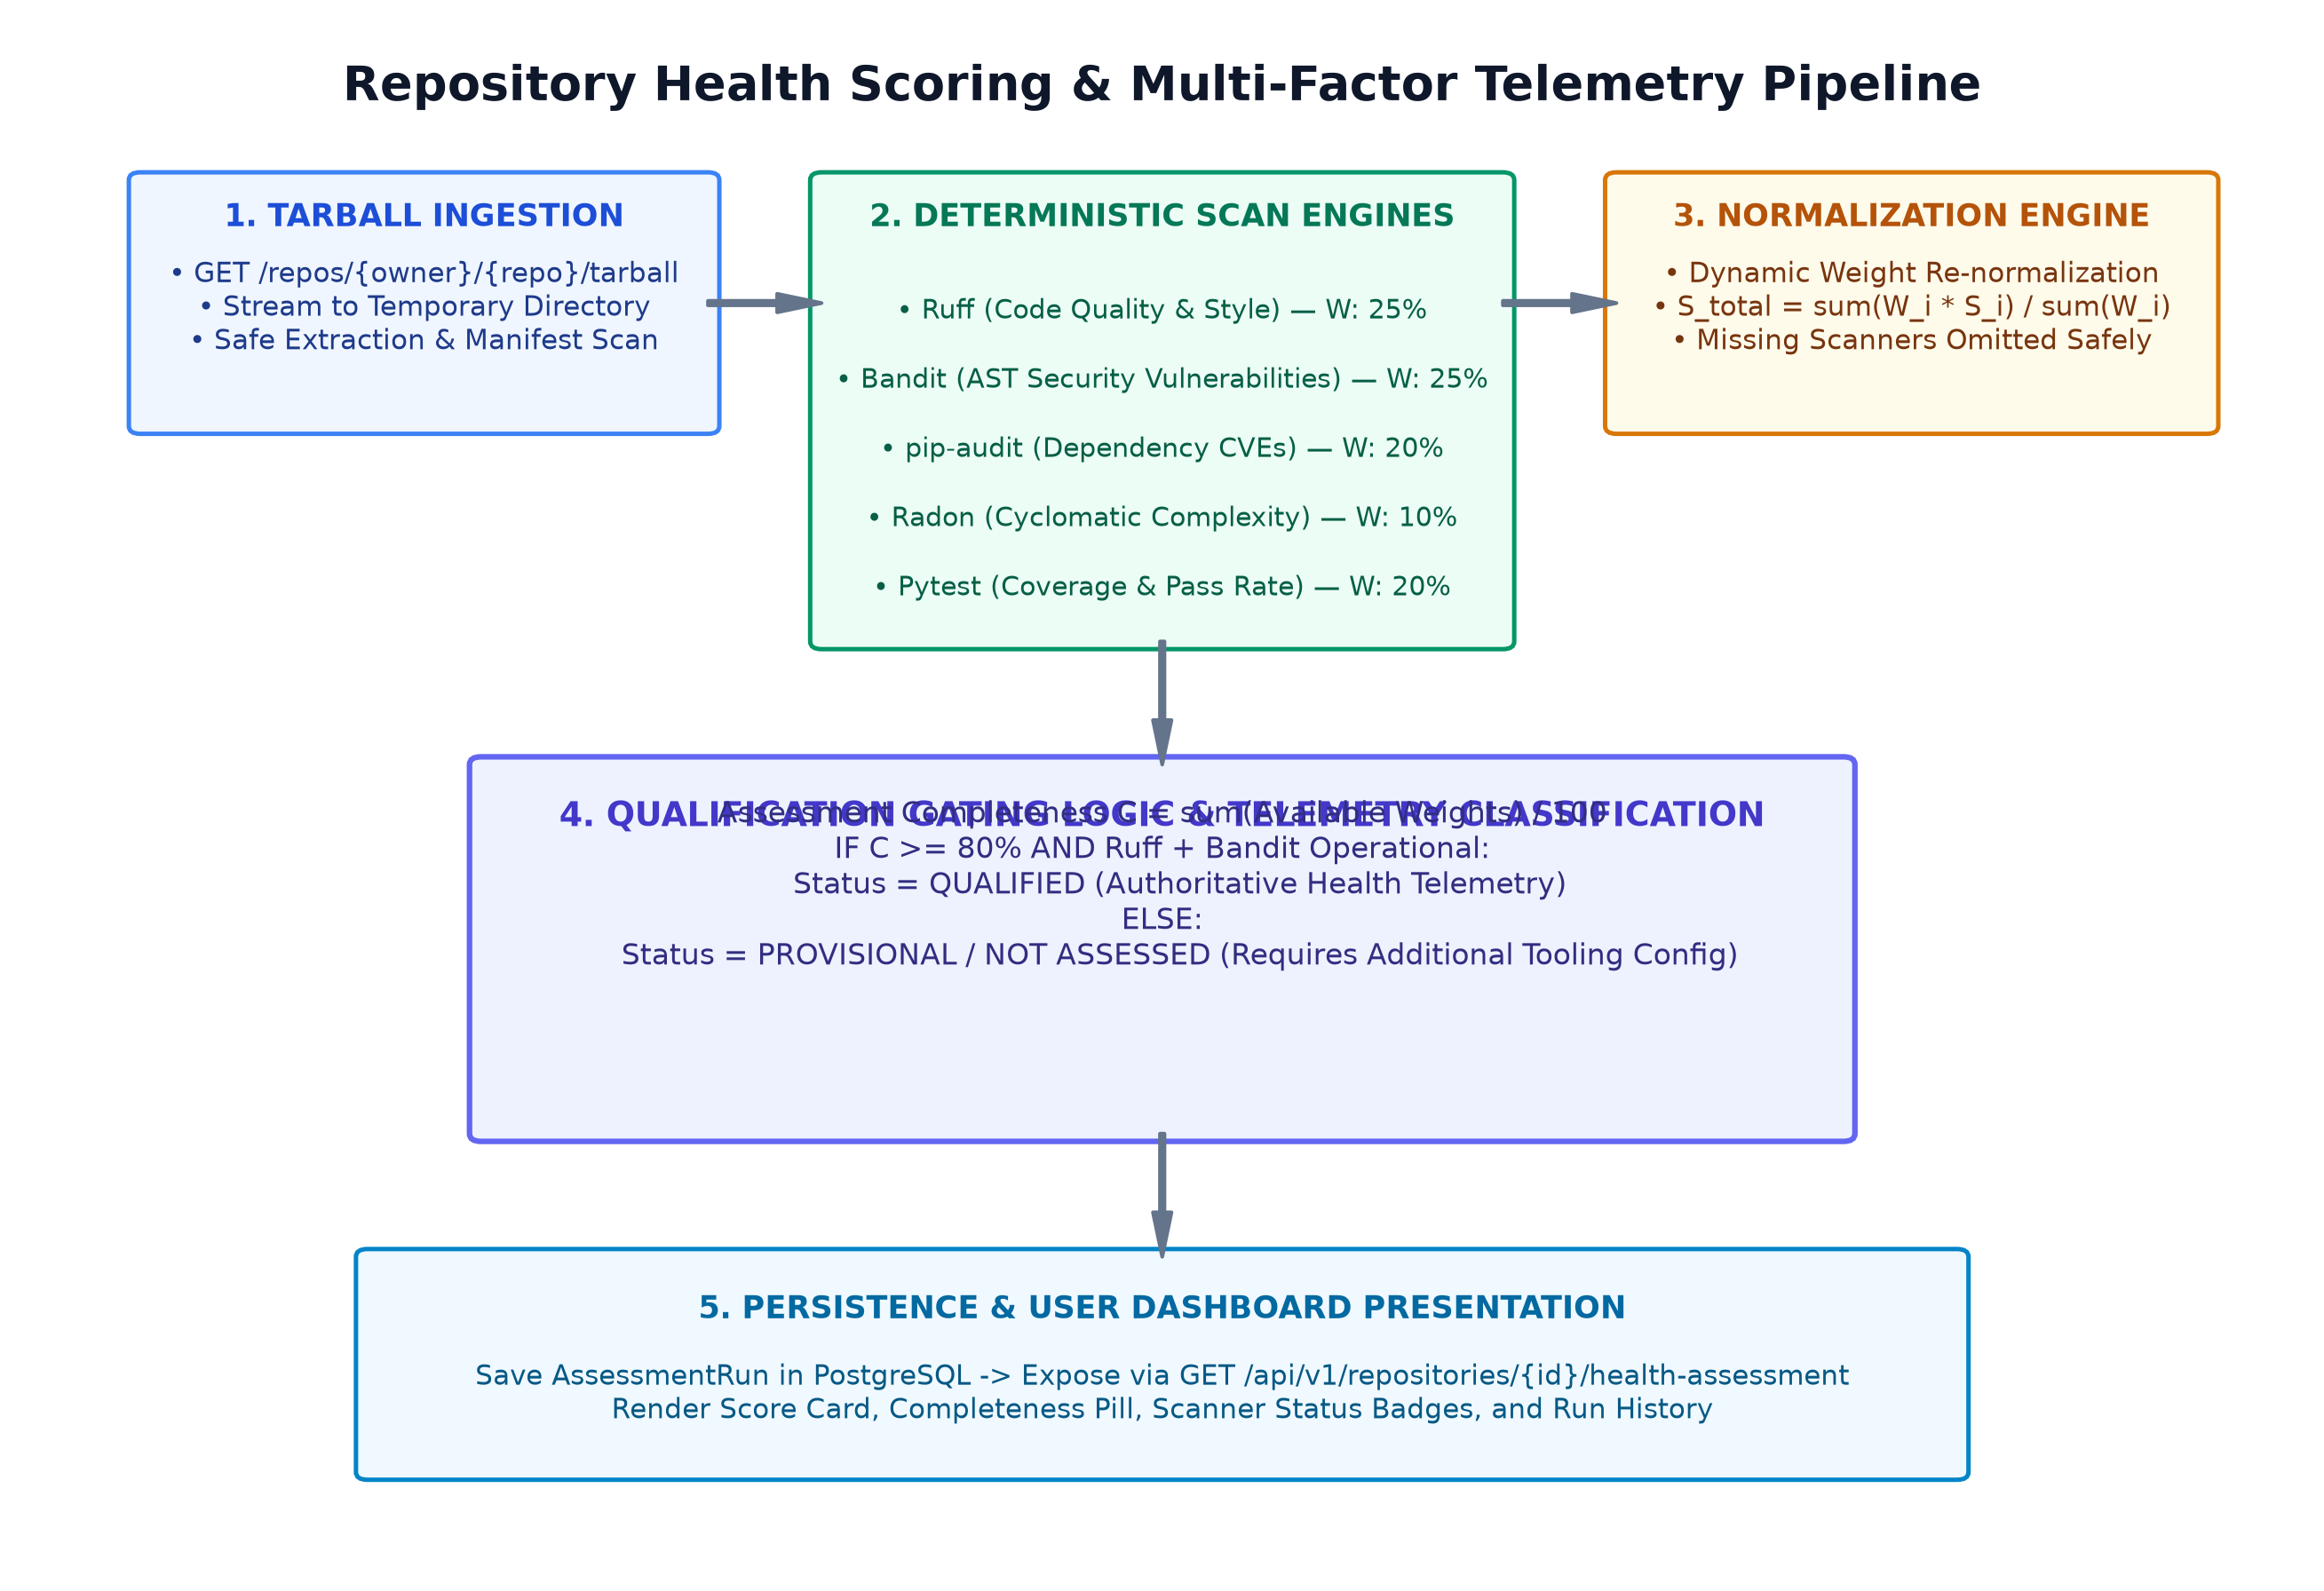
\includegraphics[width=0.92\textwidth]{images/workflows/health_assessment_workflow.png}
    \caption{Multi-Factor Health Telemetry and Dynamic Scoring Pipeline}
    \label{fig:health-workflow}
\end{figure}

\section{Enterprise Security Posture Governance Framework}
\label{sec:posture-framework}

To eliminate organizational blindspots beyond source code text, MergeMind evaluates 43 deterministic policy checks across four foundational domains, as illustrated in Figure~\ref{fig:security-architecture}:
\begin{enumerate}
    \item \textbf{Branch Protection (12 checks):} Validates mandatory PR reviews, dismissal of stale reviews, CODEOWNERS approval enforcement, admin bypass restrictions, status check enforcement, force push blocking, and signed commit requirements.
    \item \textbf{Security Features (9 checks):} Audits SECURITY.md presence, Dependabot alerts, Dependabot updates, CodeQL SARIF workflows, secret scanning, push protection, and critical CVE counts.
    \item \textbf{Access Control (8 checks):} Audits public repo exposure risks, admin count hygiene ($\le 3$), outside collaborators, write-enabled deploy keys, stale deploy keys, and plaintext webhook URLs.
    \item \textbf{Repository Settings \& Actions (14 checks):} Checks public wiki settings, issue tracking, README/LICENSE compliance, Actions execution permissions, read-only GITHUB\_TOKEN scopes, and Actions PR approval bans.
\end{enumerate}

\begin{figure}[htbp]
    \centering
    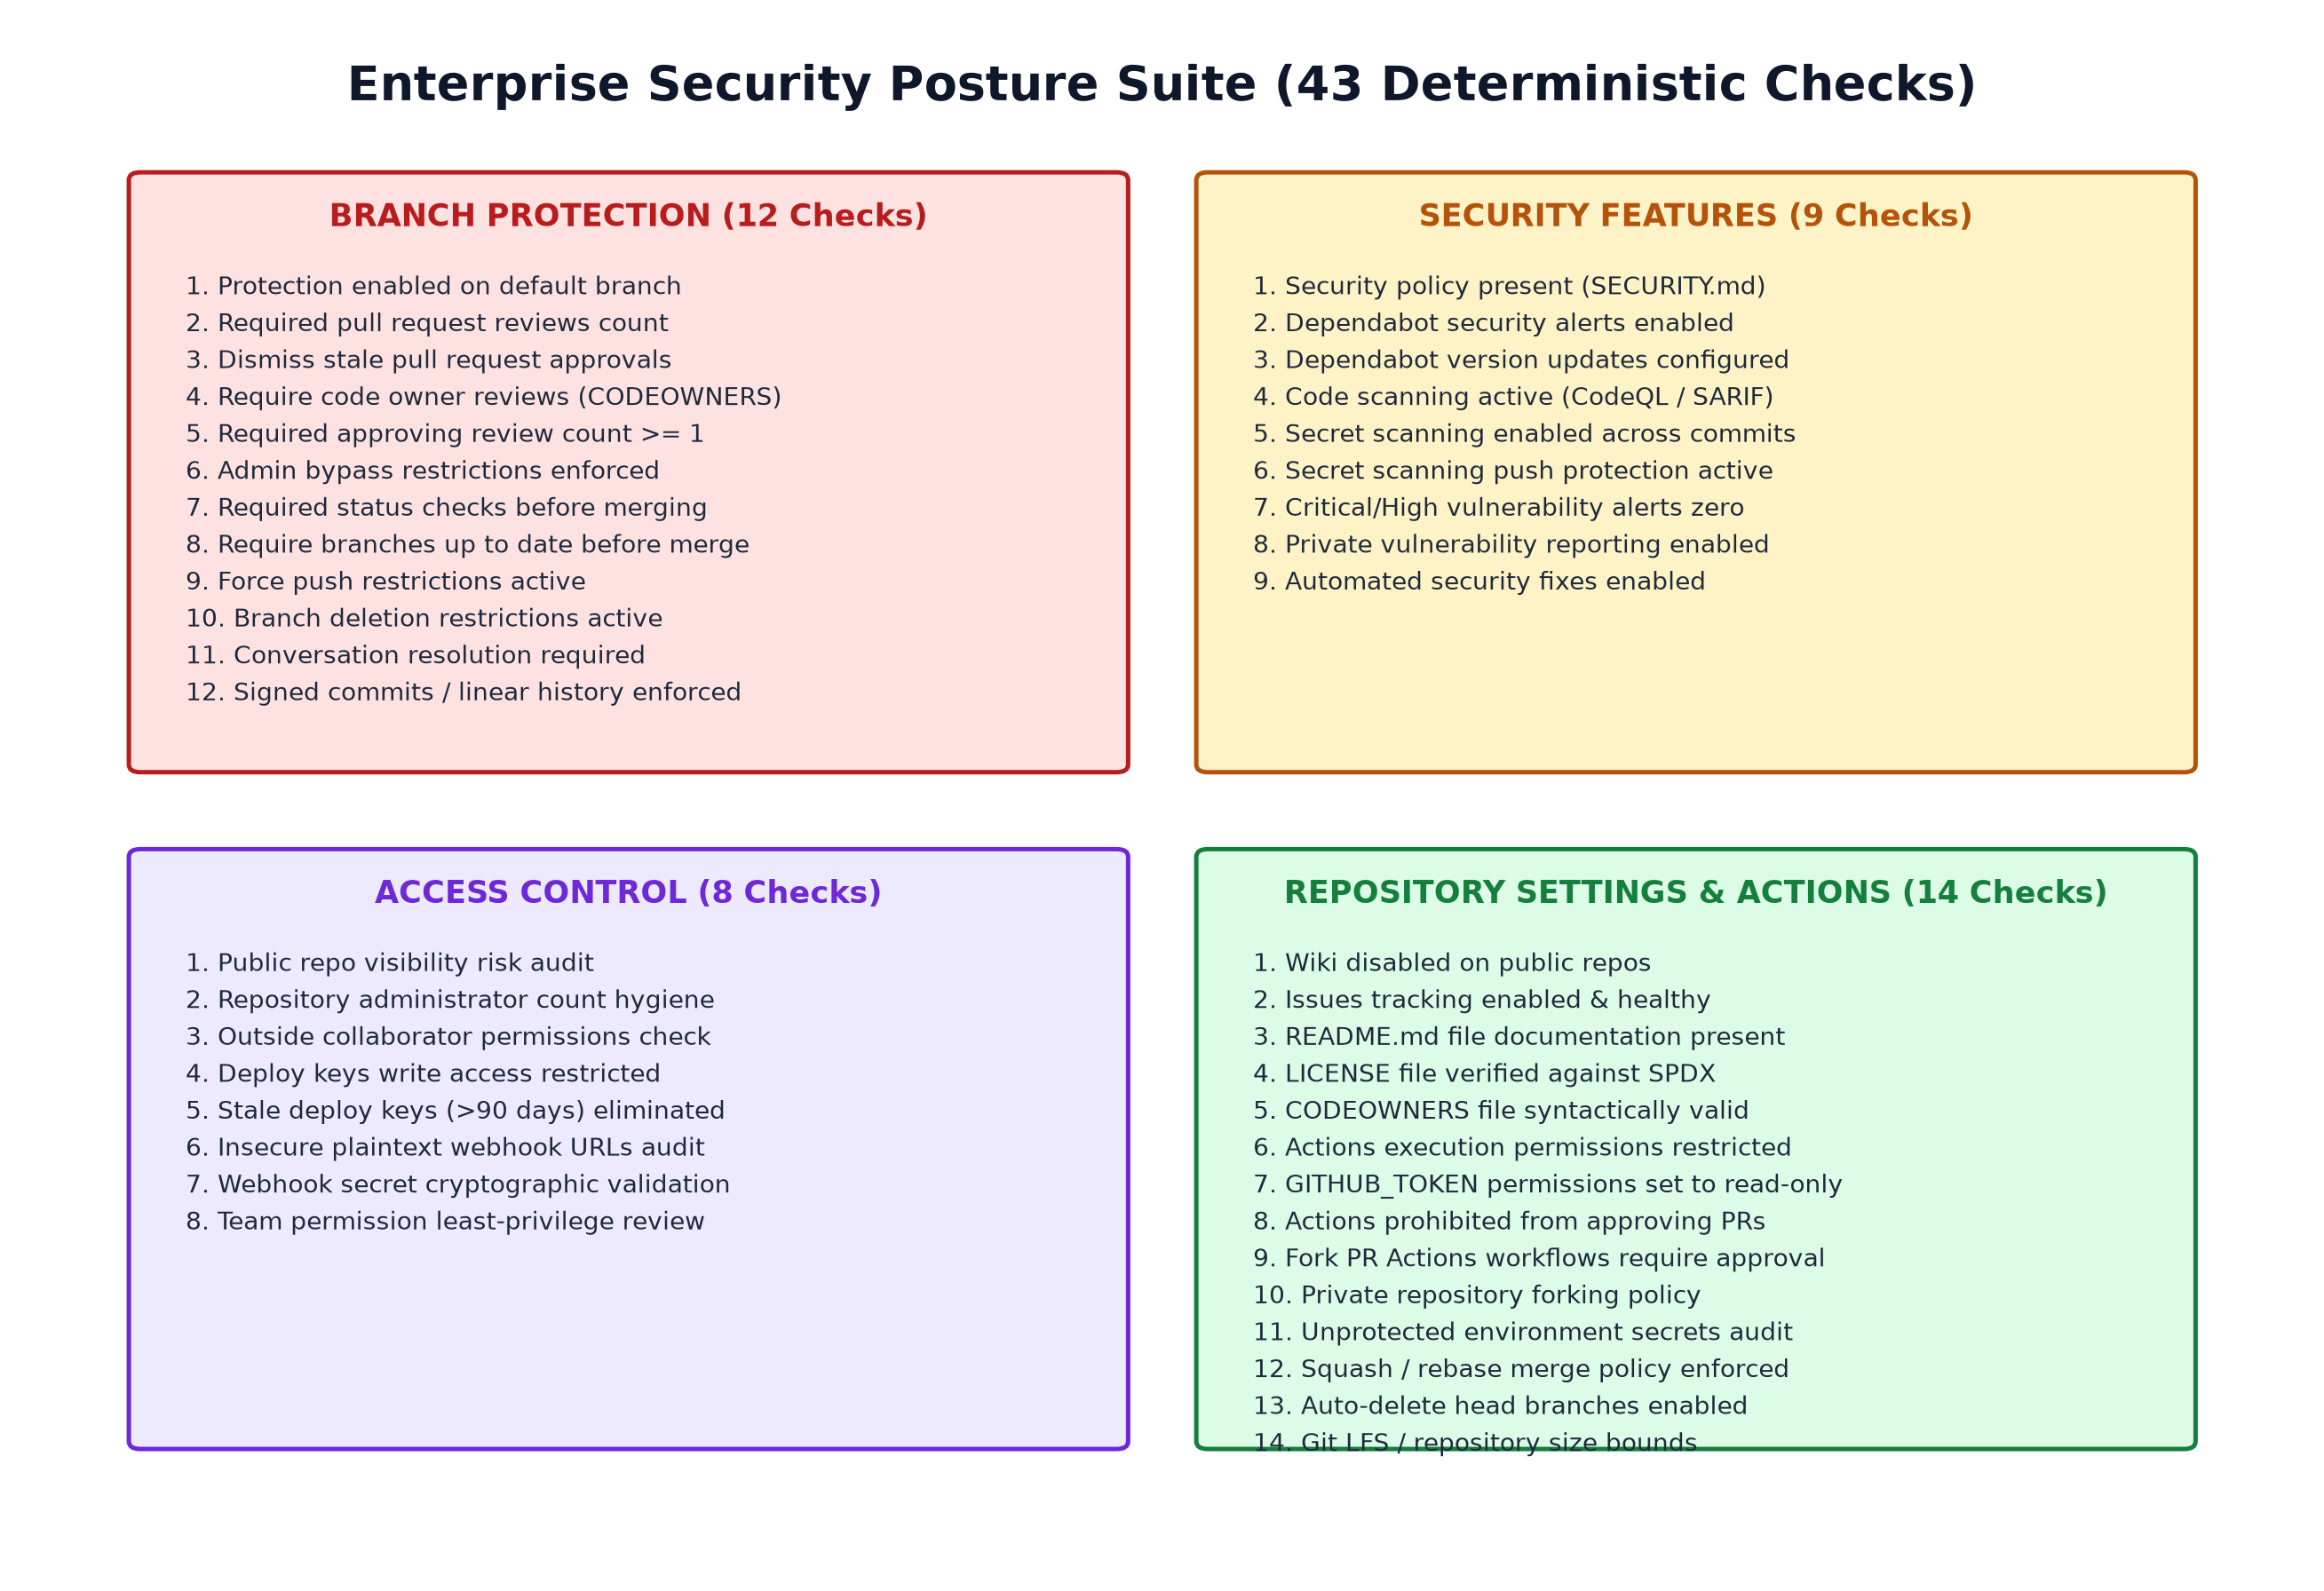
\includegraphics[width=0.92\textwidth]{images/architecture/security_architecture.png}
    \caption{Enterprise Security Posture Suite Architecture (43 Deterministic Policy Checks across 4 Domains)}
    \label{fig:security-architecture}
\end{figure}

The composite Security Posture Index (SPI) is mathematically computed as:

\begin{equation}
\text{SPI} = \left( \frac{K_1}{12} \times 0.35 + \frac{K_2}{9} \times 0.30 + \frac{K_3}{8} \times 0.20 + \frac{K_4}{14} \times 0.15 \right) \times 100
\label{eq:spi-formula}
\end{equation}
where $K_1, K_2, K_3, K_4$ represent passing check counts in each respective domain.

\section{AI Remediation and Docker Sandbox Verification Architecture}
\label{sec:remediation-design}

When a CI/CD workflow fails, MergeMind executes an automated closed-loop remediation pipeline shown in Figure~\ref{fig:remediation-workflow}:
\begin{enumerate}
    \item \textbf{Regex Token Scrubbing:} Strips \texttt{ghp\_*}, AWS secret keys, and Bearer tokens from raw console traces.
    \item \textbf{AST Stack Frame Extraction:} Pinpoints the exact failing source file, line number, and broken function symbol.
    \item \textbf{Gemini 3.6 Flash Patch Synthesis:} Injects sanitized context to generate a standard Unified Diff patch.
    \item \textbf{AST Syntax Validation:} Evaluates the candidate patch via Python's \texttt{ast.parse()} to guarantee syntactic validity.
    \item \textbf{Isolated Docker Sandbox Verification:} Applies the diff inside an ephemeral unprivileged container and re-runs Pytest.
    \item \textbf{Automated Draft PR Creation:} Upon exit code 0, automatically authors a GitHub Draft PR containing the fix and explanation.
\end{enumerate}

\begin{figure}[htbp]
    \centering
    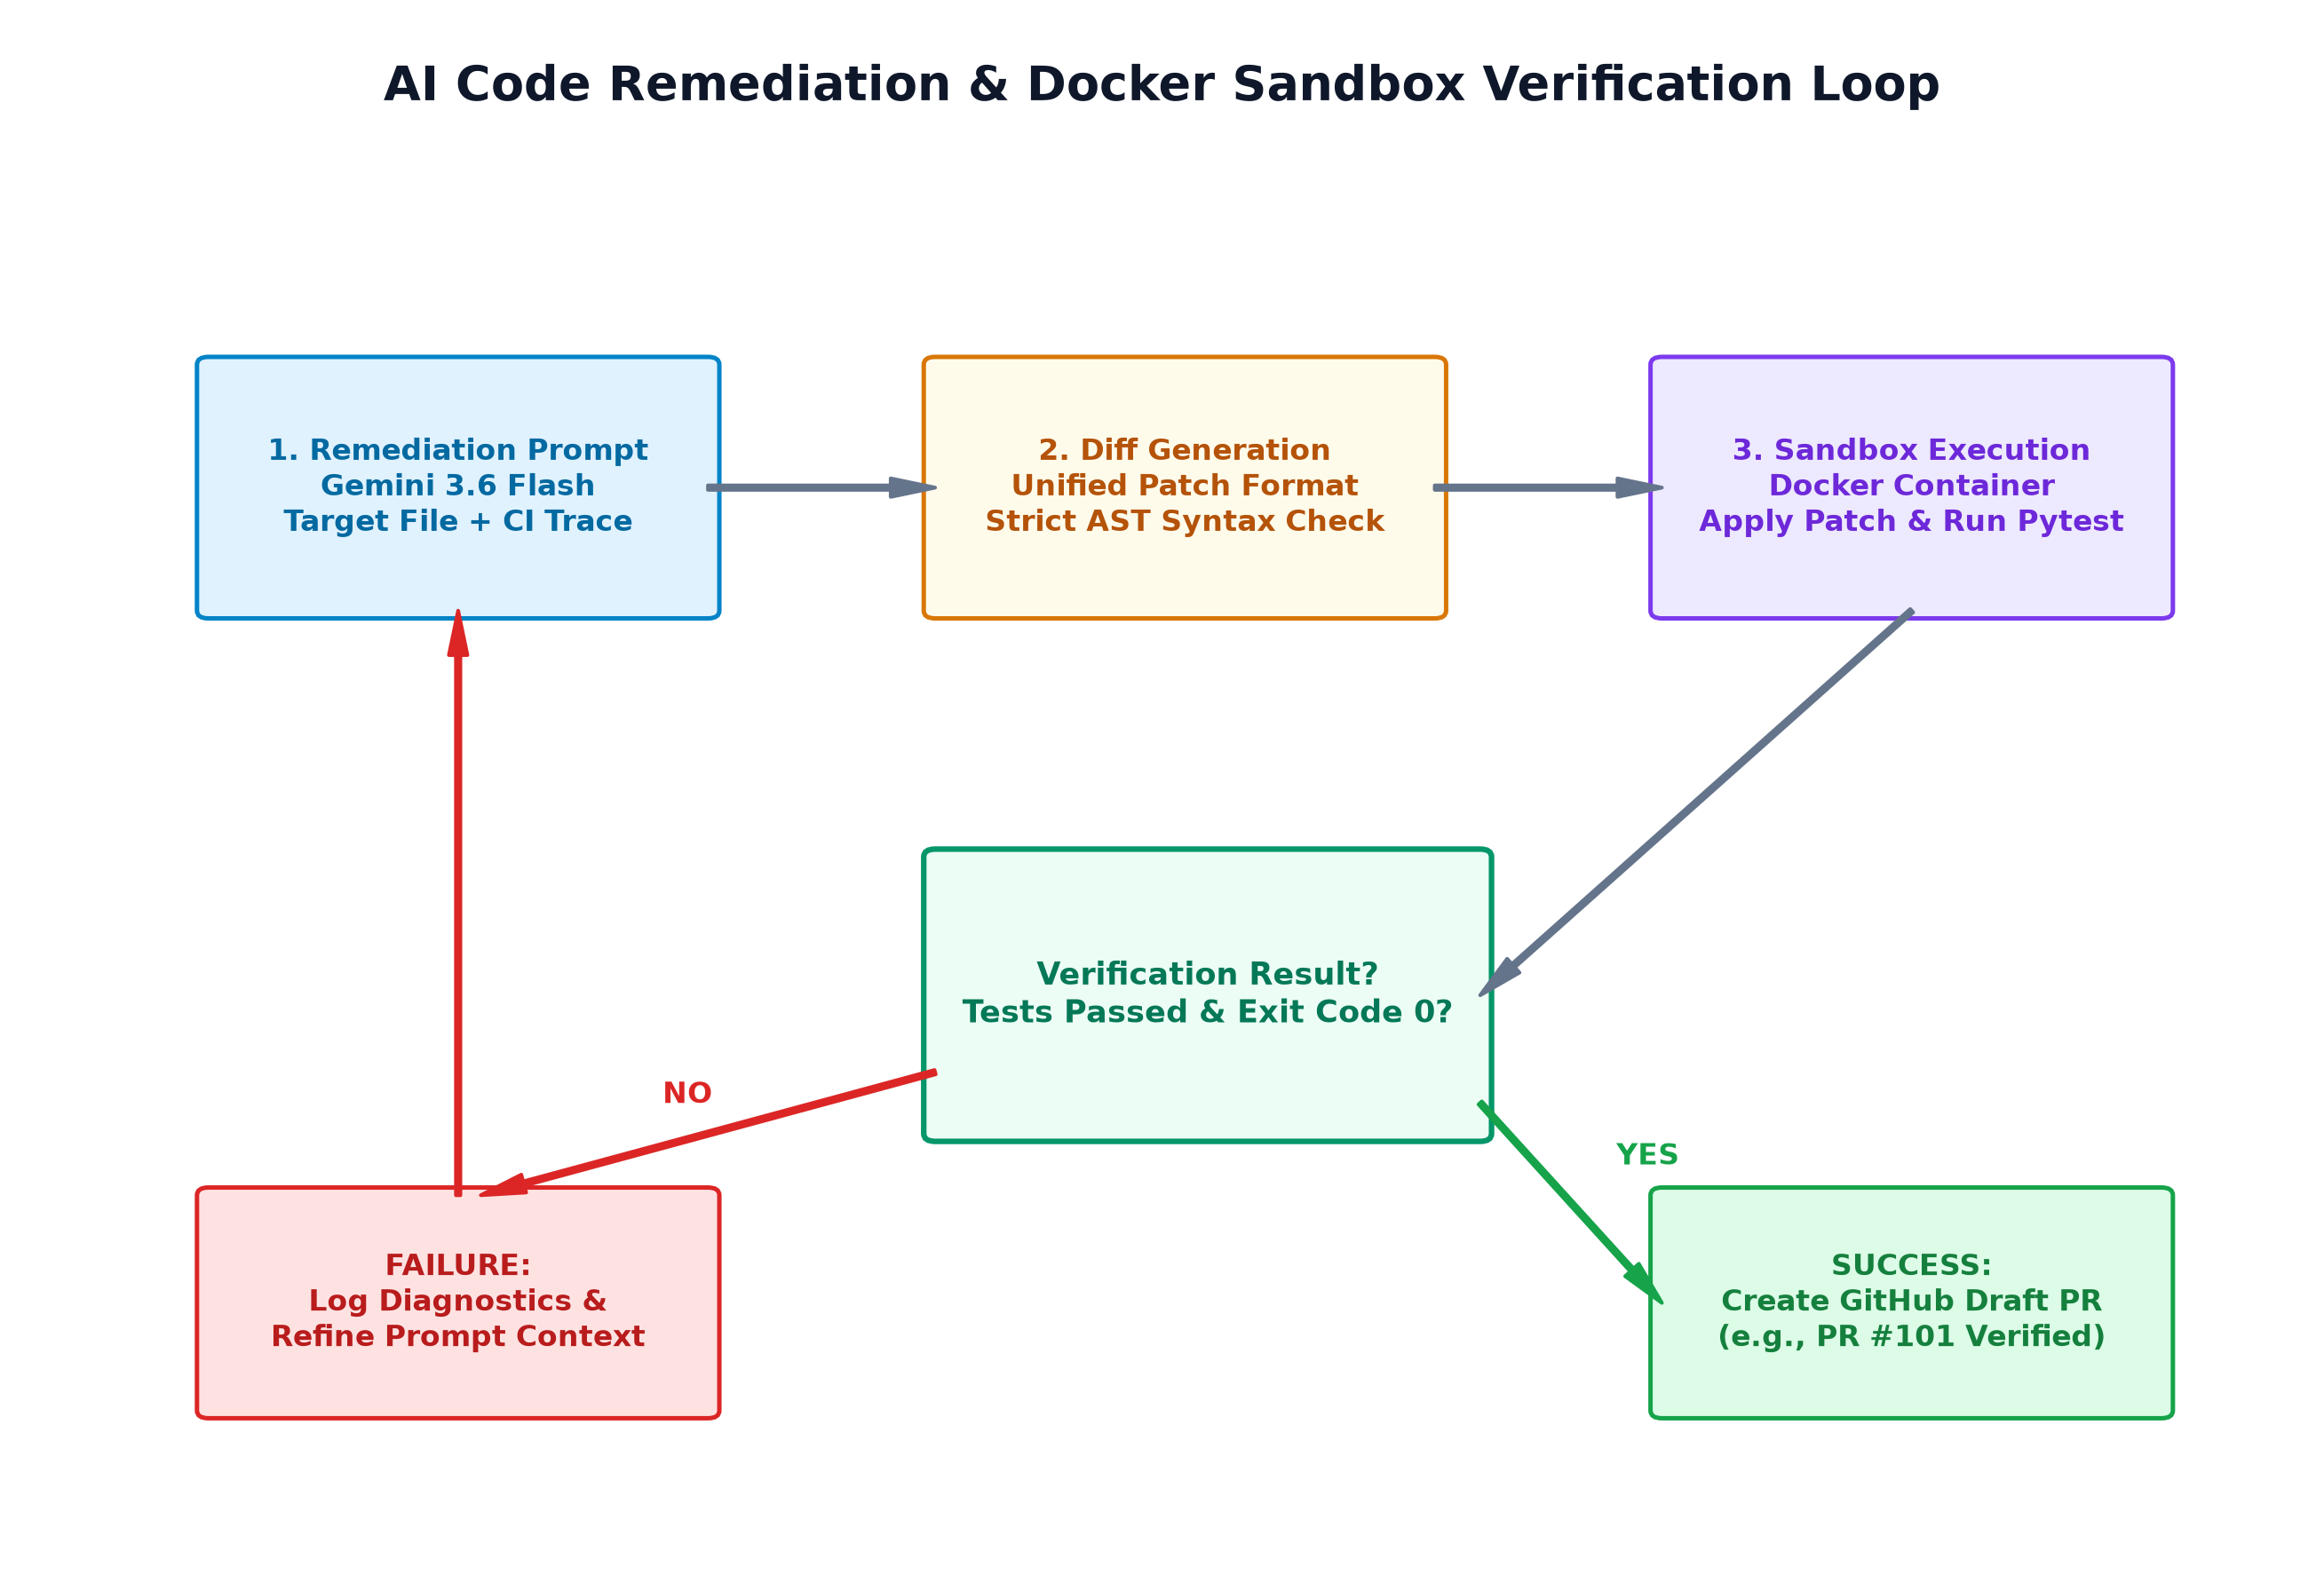
\includegraphics[width=0.92\textwidth]{images/workflows/remediation_verification_workflow.png}
    \caption{AI Code Remediation and Docker Sandbox Verification Execution Loop}
    \label{fig:remediation-workflow}
\end{figure}

\section{Database and Container Deployment Topology}
\label{sec:db-deploy-topology}

The persistence layer models repositories, health runs, CI failures, remediation diffs, and PR reviews. Figure~\ref{fig:database-er} displays the complete Entity-Relationship schema diagram, while Figure~\ref{fig:deployment-topology} illustrates the containerized deployment topology orchestrating frontend, backend, and PostgreSQL database within an isolated bridge network.

\begin{figure}[htbp]
    \centering
    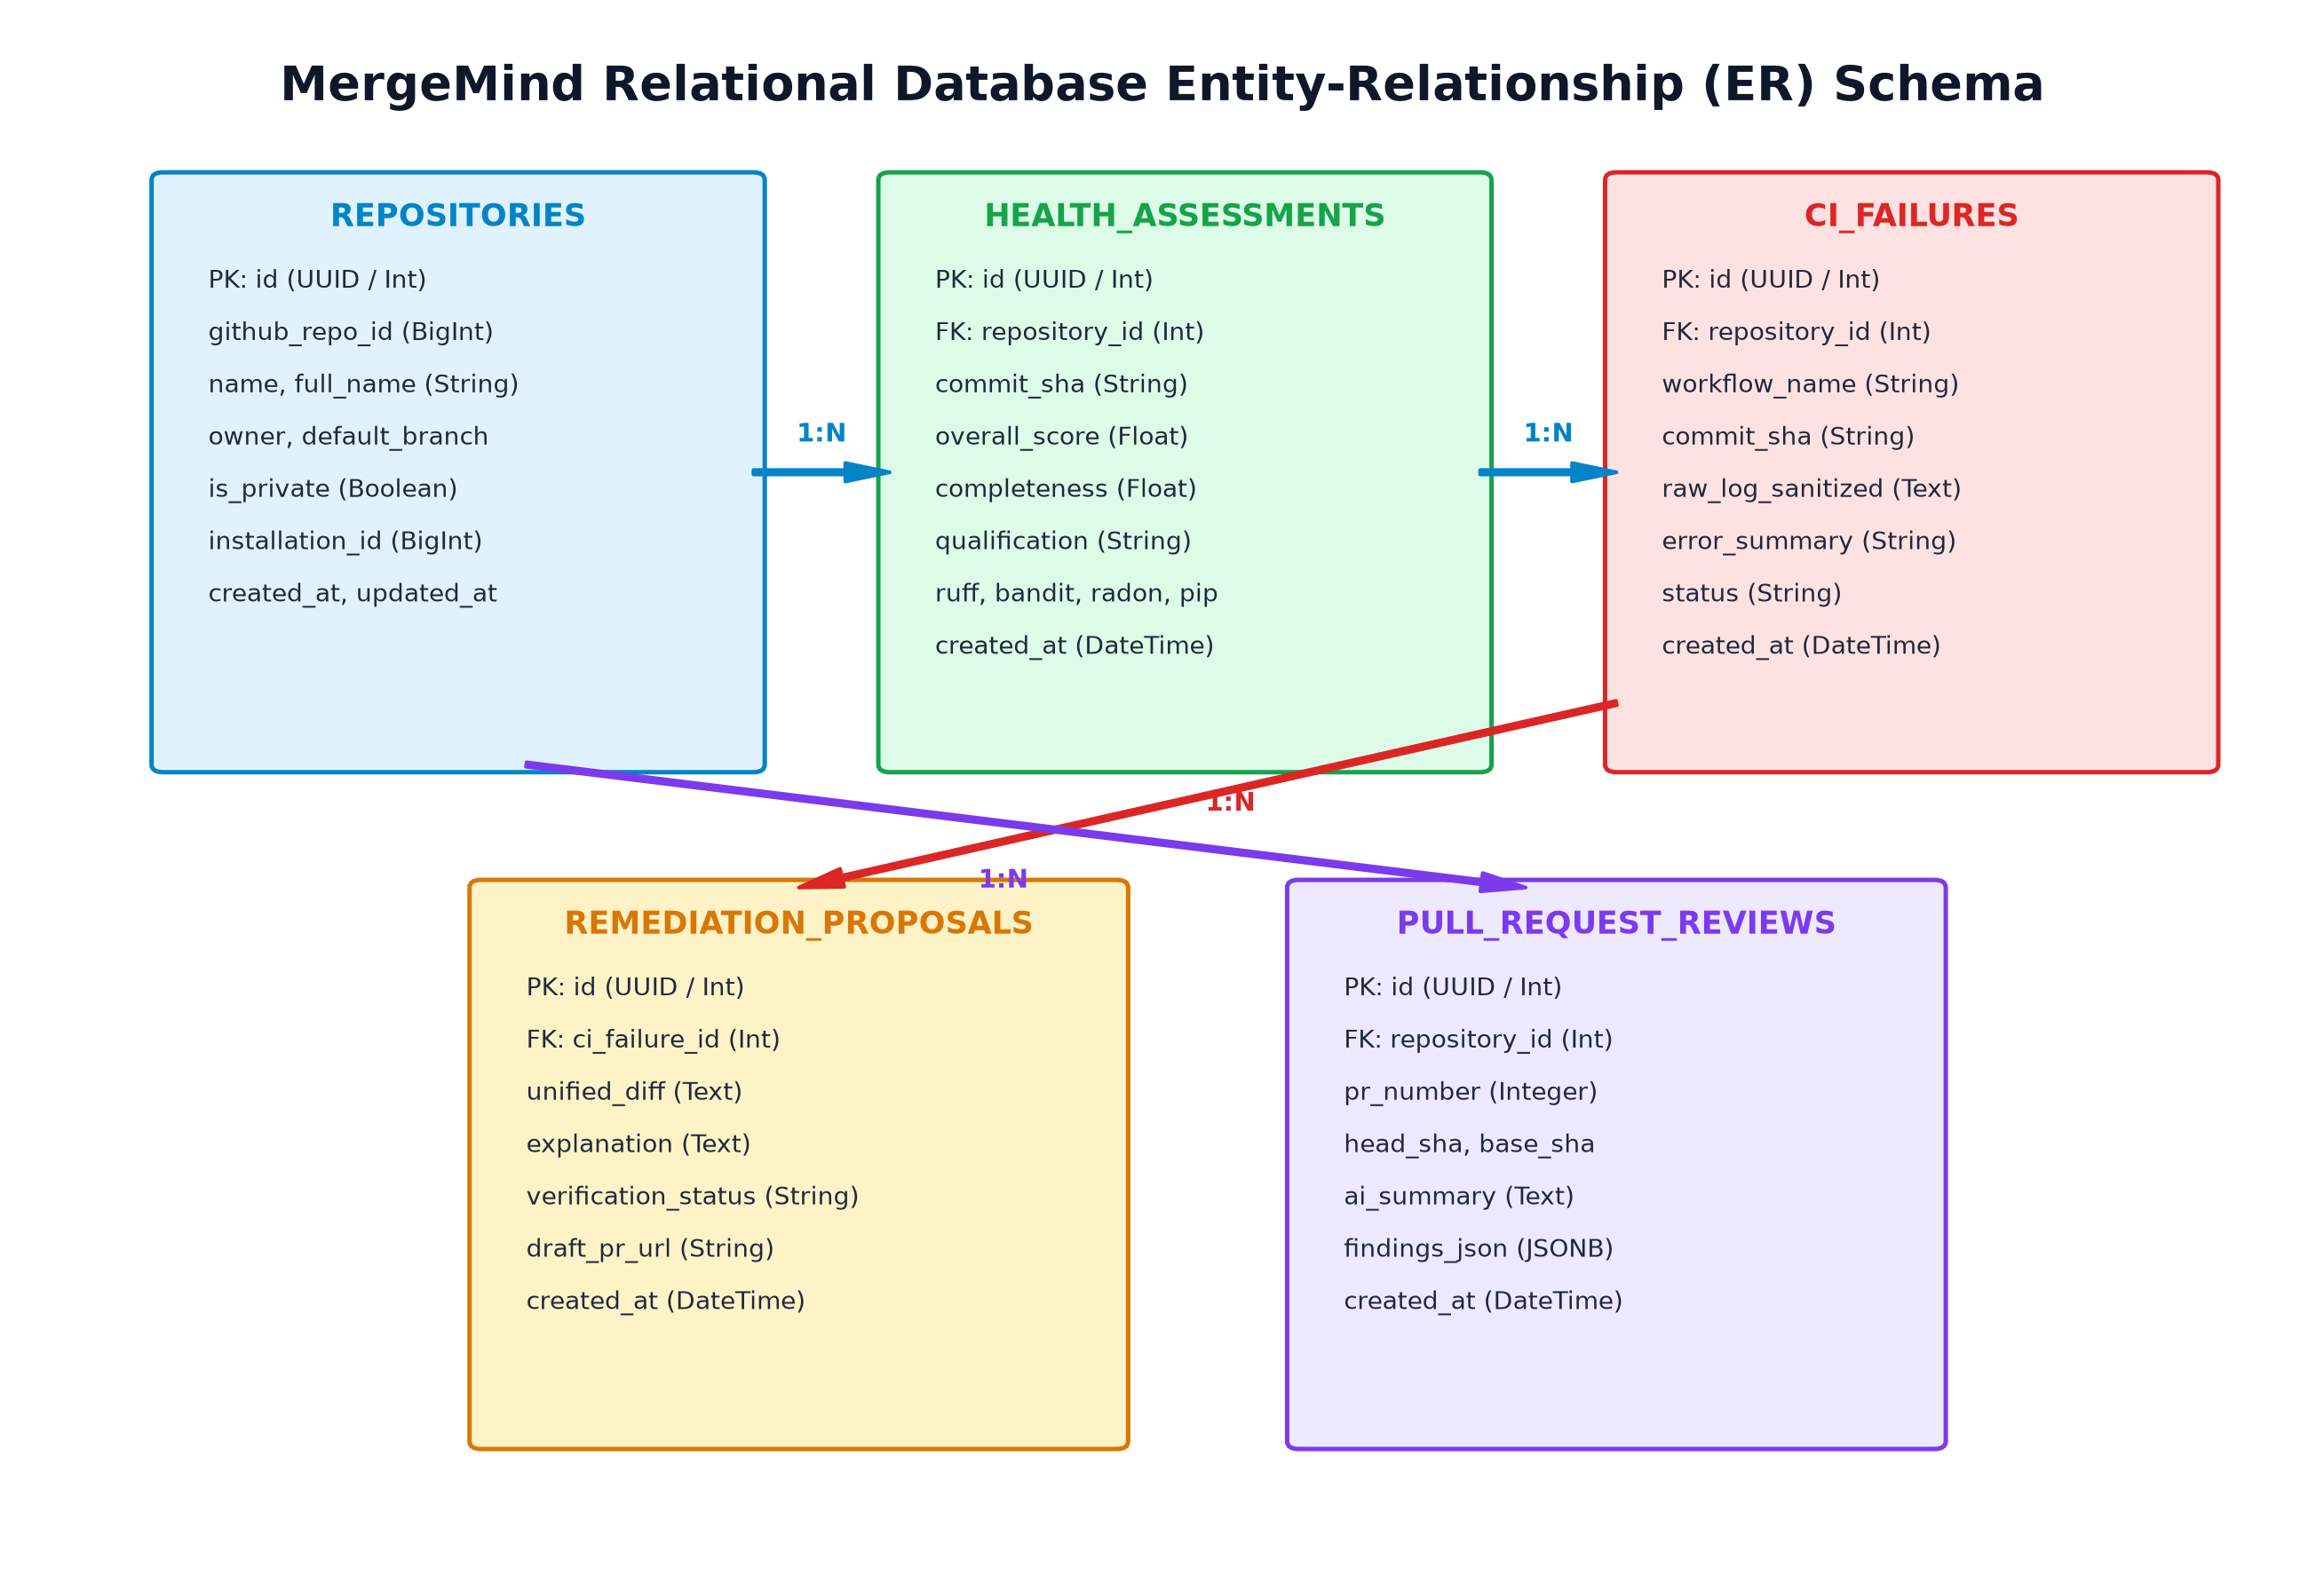
\includegraphics[width=0.92\textwidth]{images/database/database_er_diagram.png}
    \caption{MergeMind Relational Database Entity-Relationship (ER) Schema Diagram}
    \label{fig:database-er}
\end{figure}

\begin{figure}[htbp]
    \centering
    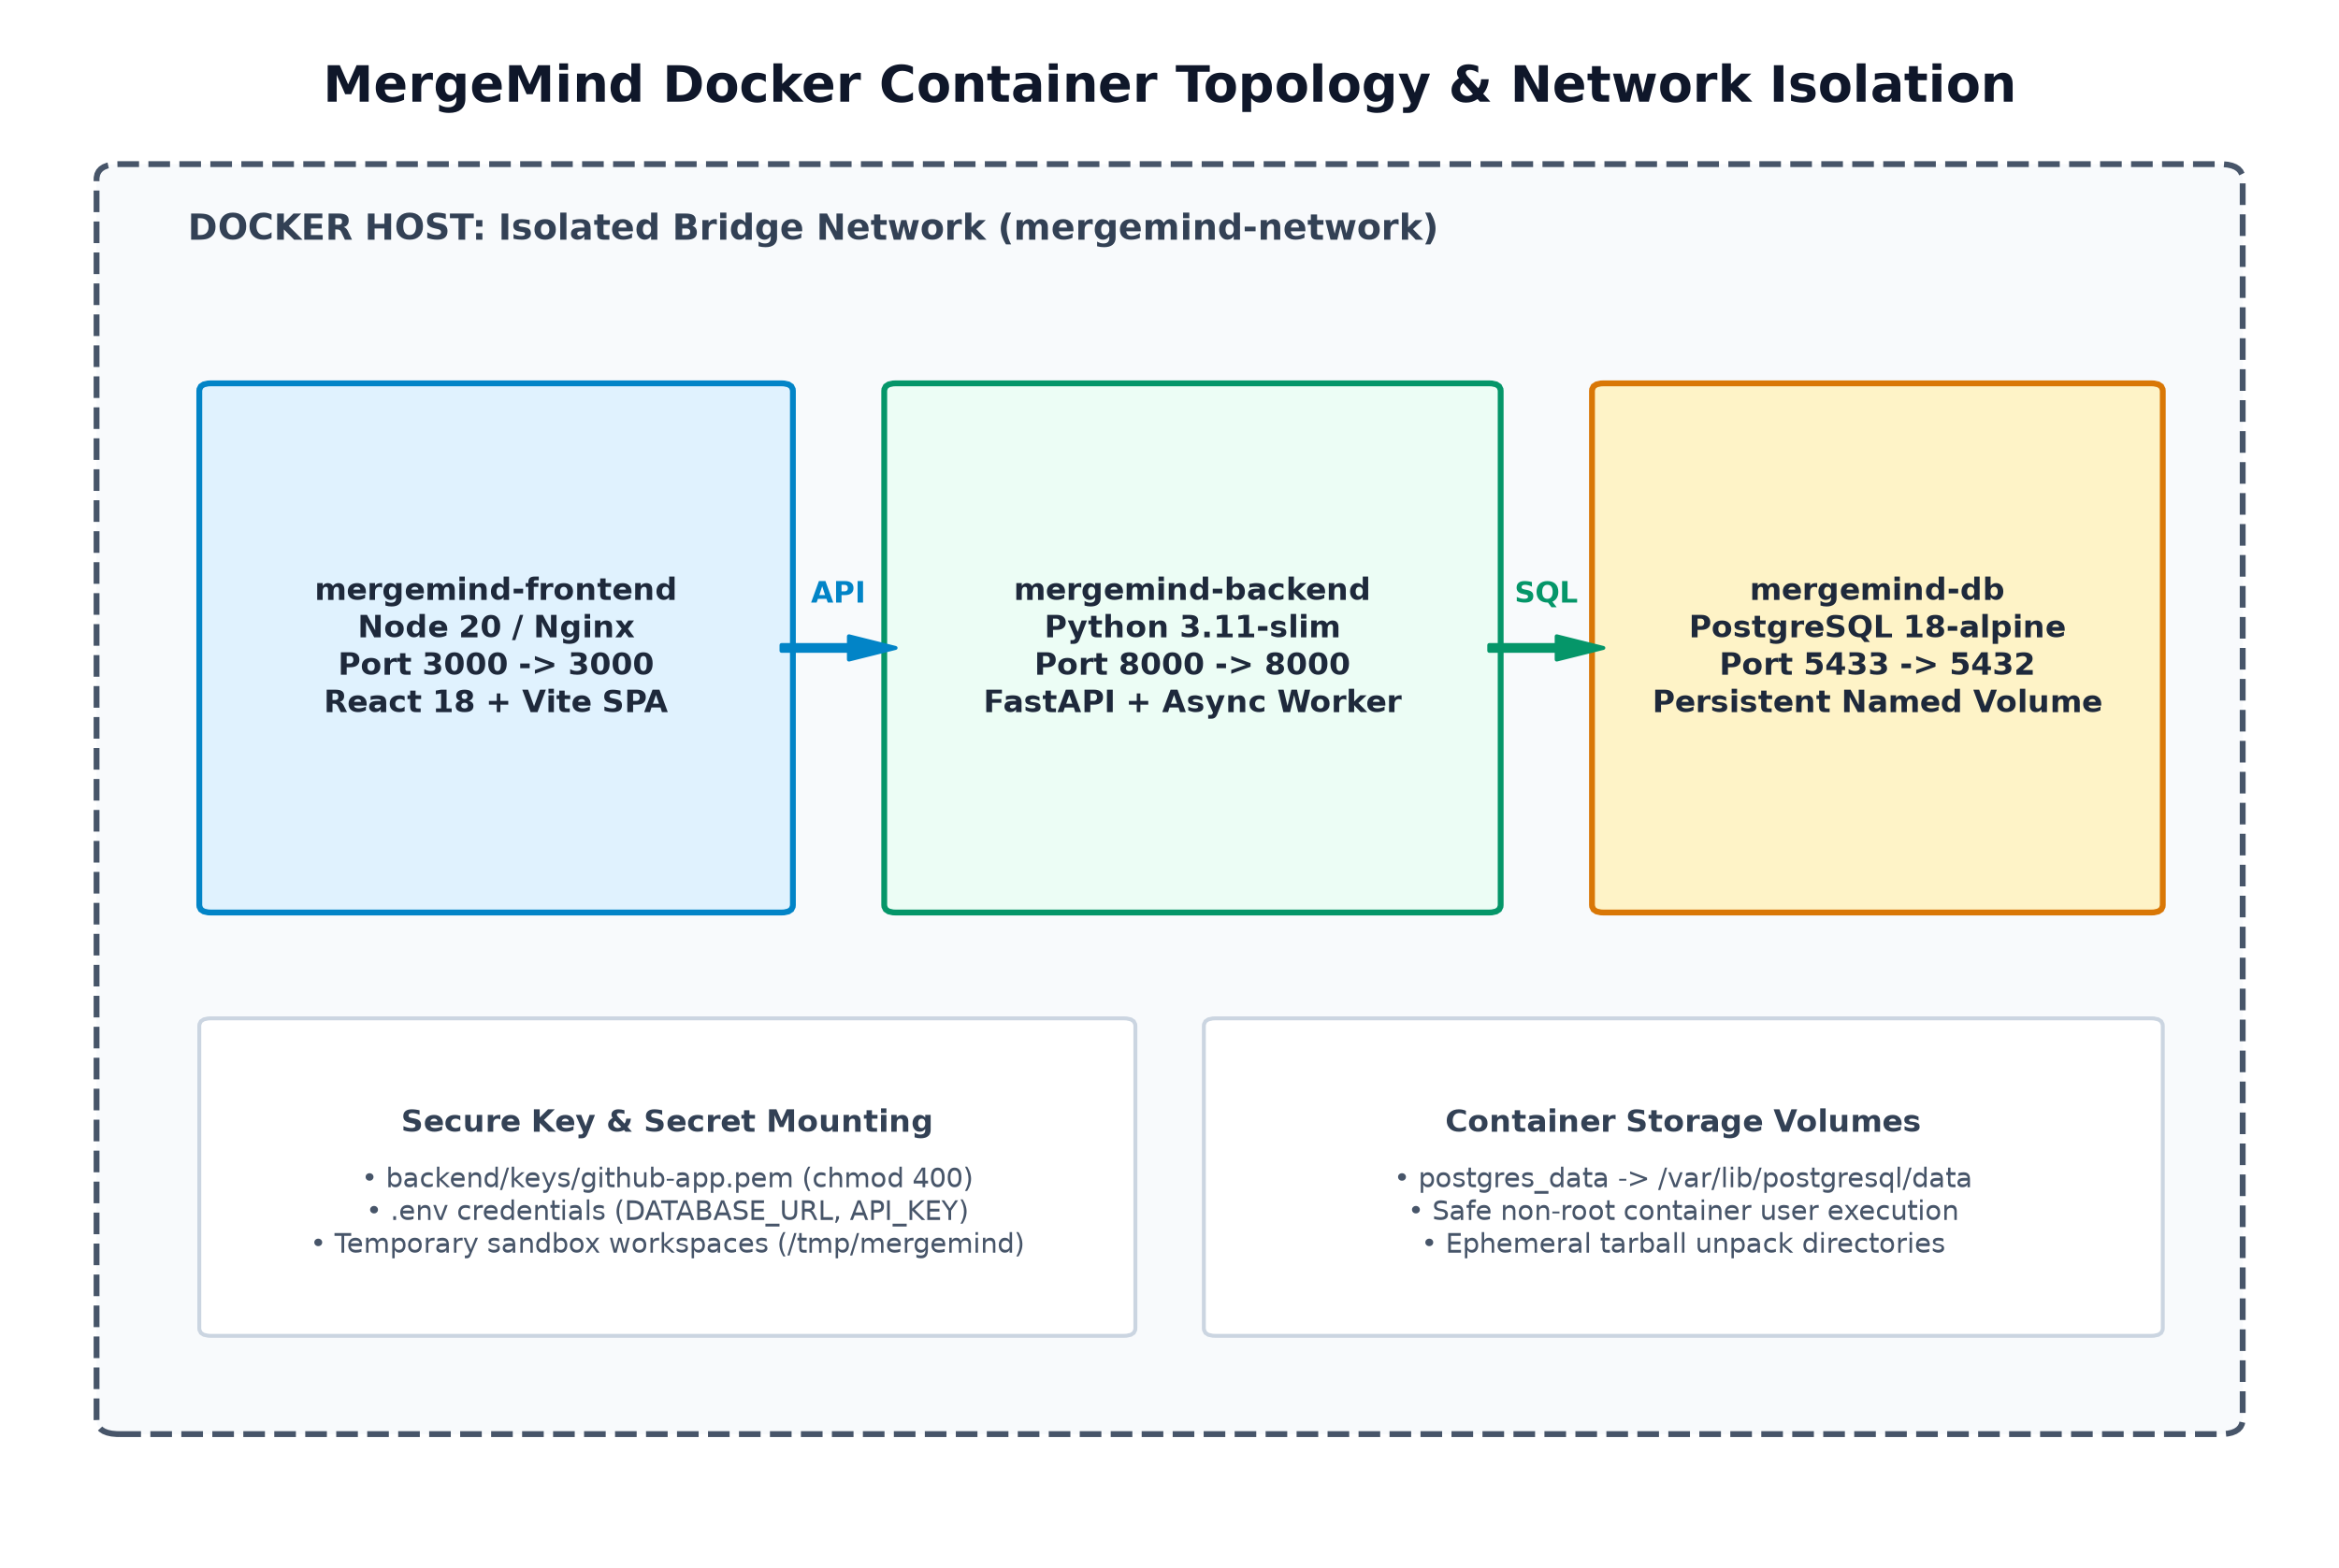
\includegraphics[width=0.88\textwidth]{images/architecture/deployment_topology.png}
    \caption{Docker Container Deployment Topology and Network Isolation}
    \label{fig:deployment-topology}
\end{figure}
